\documentclass[aspectratio=169, table, 12pt]{beamer}

% Preamble bersama seluruh slide mata kuliah ini.
% Dipanggil dari slides/sessionXX/sessionXX.tex tepat sesudah baris
% \documentclass[aspectratio=169, table, 12pt]{beamer}
% Paket tambahan yang hanya dibutuhkan satu sesi ditulis di berkas sesi itu.

\usepackage{colortbl}
\usepackage{xcolor}
\usepackage{listings}
\usepackage{tabularx}
\usepackage{booktabs}
\usepackage{tikz}
\usepackage{pgfplots}
\pgfplotsset{compat=1.18}
\usetikzlibrary{arrows.meta, positioning, calc, fit, shapes.geometric,
	shapes.multipart, backgrounds, matrix, chains, trees}

\makeatletter
\def\input@path{{../theme/}}
\makeatother
\graphicspath{{../theme/}{../../figures/}}
\usetheme{Pradita}

\definecolor{praditagreen}{RGB}{37, 113, 71}

% Tema membuat garis tabel berwarna putih. Dikembalikan agar tabel terbaca.
\arrayrulecolor{black}
\setlength{\arrayrulewidth}{0.5pt}

\lstdefinelanguage{yaml}{
	basicstyle=\ttfamily\scriptsize,
	keywordstyle=\color{blue}\bfseries,
	commentstyle=\color{gray}\itshape,
	stringstyle=\color{red},
	showstringspaces=false,
	breaklines=true,
	frame=lines,
	numbers=none,
	backgroundcolor=\color{lightgray!10},
	tabsize=2,
	morecomment=[l]{\#}
}

\lstdefinelanguage{json}{
	basicstyle=\ttfamily\scriptsize,
	stringstyle=\color{red},
	commentstyle=\color{gray},
	breaklines=true,
	showstringspaces=false,
	tabsize=2,
	numbers=none,
	frame=lines,
	backgroundcolor=\color{lightgray!10},
	string=[s]{"}{"}
}

\lstdefinelanguage{bash}{
	keywords={},
	basicstyle=\ttfamily\scriptsize,
	ndkeywords={docker, kubectl, helm, curl, git, terraform},
	ndkeywordstyle=\color{purple}\bfseries,
	sensitive=true,
	commentstyle=\color{gray},
	numbers=none,
	breaklines=true,
	frame=lines,
	backgroundcolor=\color{lightgray!10},
	tabsize=2,
	comment=[l]{\#},
	showstringspaces=false
}

\lstdefinelanguage{http}{
	keywords={GET, POST, PUT, PATCH, DELETE, HEAD, OPTIONS, HTTP},
	basicstyle=\ttfamily\scriptsize,
	keywordstyle=\color{blue}\bfseries,
	sensitive=true,
	numbers=none,
	breaklines=true,
	frame=lines,
	backgroundcolor=\color{lightgray!10},
	tabsize=2,
	showstringspaces=false
}

\subtitle{IT40713 · Cloud-Native \& Microservices Architecture}
\author{\textbf{Alfa Yohannis}}


\title{\Huge Peta Jalan Modernisasi\\ \vspace{10pt} dan Tata Kelola Cloud}

\begin{document}

\frame{\titlepage}

\begin{frame}
  \frametitle{Isi Pertemuan}
  \vspace{14pt}
  \begin{columns}[t]
    \column{0.5\textwidth}
    {\small\tableofcontents[sections={1-4}]}

    \column{0.5\textwidth}
    {\small\tableofcontents[sections={5-8}]}
  \end{columns}
\end{frame}

\begin{frame}{\hfill}
  \centering
  \Huge{\textbf{Apa yang dimodernisasi\\lebih dulu, berapa biayanya,\\dan bagaimana risikonya\\dikendalikan?}}
\end{frame}

\section{Tujuan dan Konteks}

\begin{frame}{\hfill}
  \centering
  \Huge{\textbf{Tujuan dan Konteks}}
\end{frame}

\begin{frame}{{\Large Tujuan Pembelajaran}}
  \vspace{10pt}
  \begin{itemize}
    \item Menyusun urutan modernisasi bertahap dengan pola \textit{strangler fig}.
    \item Merancang \textit{guardrail} tata kelola \textit{cloud} untuk biaya, keamanan, dan lokasi
          data.
    \item Mempertahankan peta jalan modernisasi di depan pemangku kepentingan dengan metrik yang
          terukur.
  \end{itemize}
\end{frame}

\begin{frame}{{\Large Permintaan Direksi Medikara Health}}
  \vspace{10pt}
  \begin{itemize}
    \item Direksi meminta satu dokumen untuk tiga pertanyaan: apa dulu, berapa biaya, bagaimana
          risiko.
    \item Satu semester menghasilkan banyak artefak, dari lokasi data sampai model operasi.
    \item Direktur keuangan: tumpukan artefak belum tentu sebuah rencana.
    \item Bahan pokok: urutan bertahap, \textit{guardrail}, dan metrik kemajuan.
    \item Hasilnya menjadi bagian terakhir tonggak capstone C4, menjelang UAS.
  \end{itemize}
\end{frame}

\IfFileExists{../../figures/ch14-diagram-konsep.png}{%
\begin{frame}{{\Large Diagram Konsep Bab 14}}
  \centering
  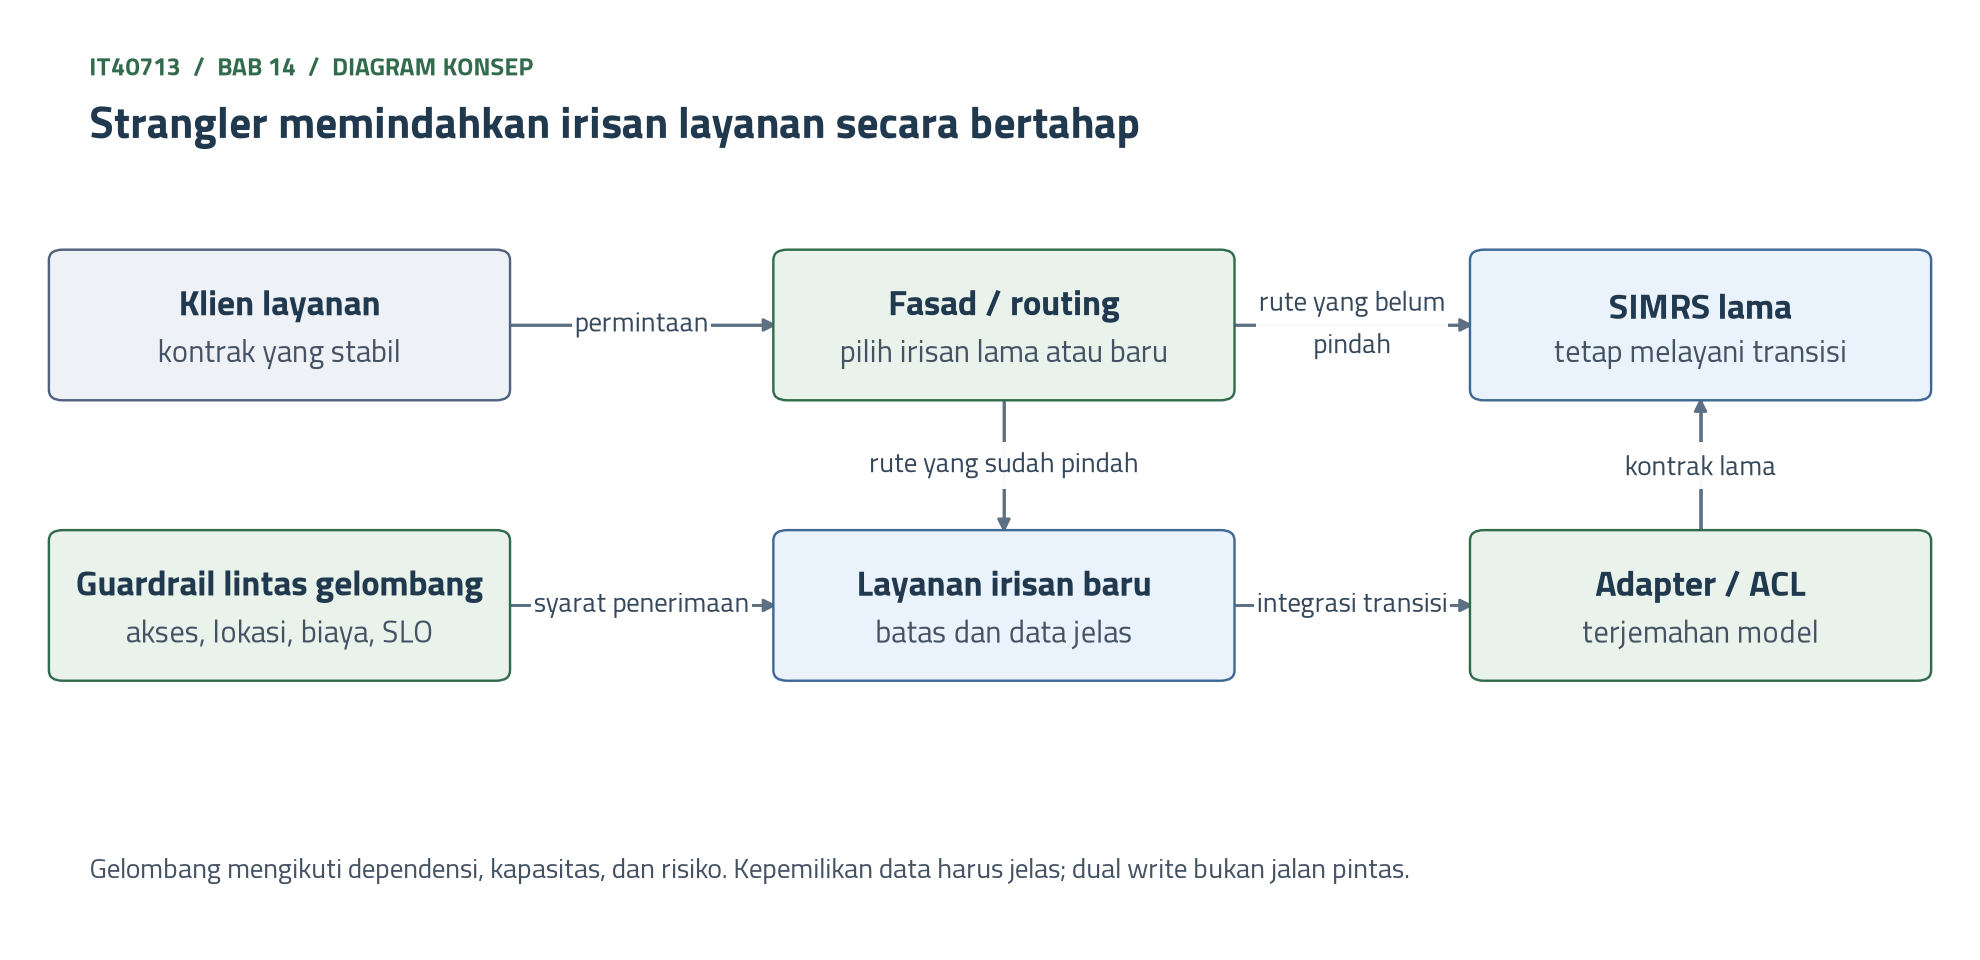
\includegraphics[width=0.96\textwidth,height=0.77\textheight,keepaspectratio]{../../figures/ch14-diagram-konsep.png}
\end{frame}
}{}

\begin{frame}{{\Large Keputusan yang Dibawa ke Peta Jalan}}
  \footnotesize
  \begin{tabularx}{\textwidth}{>{\raggedright\arraybackslash}p{1.5cm}
      >{\raggedright\arraybackslash}X}
    \hline
    \textbf{Bab} & \textbf{Keputusan} \\ \hline
    Bab 2 dan 3 & Rekam medis di \textit{region} Indonesia. Biaya SIMRS per kunjungan RS Bekasi
      Rp5.619 menjadi paling tinggi Rp4.776; Medikara+ Rp2.036 per janji temu \\ \hline
    Bab 4 & 46 aplikasi: Retire 6, Retain 5, Rehost 10, Relocate 15 (termasuk Medikara+), Repurchase
      3, Replatform 2, SIMRS diperdebatkan 5. \textit{Landing zone} 8 minggu; CCoE \\ \hline
    Bab 5 sampai 7 & Rilis Medikara+ 37 langkah manual; \textit{bounded context} jadi batas modul;
      ADR-001: SIMRS terpadu \textit{modular monolith}, janji temu calon pertama \\ \hline
    Bab 8 sampai 10 & PaaS untuk layanan baru pertama; janji temu berbasis \textit{event}; Layanan
      Identitas Pasien memiliki 31 kolom identitas \\ \hline
    Bab 11 dan 12 & SLO janji temu 99,5 persen, hasil laboratorium 99,0 persen, klaim 98,0 persen.
      Rekam medis RTO 1 jam, RPO 5 menit; biaya DR sekitar Rp724 juta per tahun \\ \hline
    Bab 13 & 52 staf TI; tim platform 6 orang; sasaran SIMRS rilis bulanan lalu mingguan \\ \hline
  \end{tabularx}
\end{frame}

\section{Pola Strangler Fig}

\begin{frame}{\hfill}
  \centering
  \Huge{\textbf{Pola Strangler Fig}}
\end{frame}

\begin{frame}{{\Large Sekaligus atau Bertahap}}
  \footnotesize
  \begin{tabularx}{\textwidth}{>{\raggedright\arraybackslash}p{2.8cm}
      >{\raggedright\arraybackslash}X >{\raggedright\arraybackslash}X}
    \hline
    \textbf{Aspek} & \textbf{Penggantian sekaligus} & \textbf{Penggantian bertahap} \\ \hline
    Titik risiko & Satu malam peralihan & Banyak langkah kecil \\ \hline
    Nilai bisnis pertama & Setelah seluruh pekerjaan selesai & Setelah irisan pertama berjalan \\
      \hline
    Kembali ke sistem lama & Sulit setelah data baru ditulis & Mudah selama rute lama ada \\ \hline
    Biaya masa transisi & Kecil & Ada fasad, penerjemah, dua sistem berjalan \\ \hline
    Pembelajaran tim & Baru terjadi saat peralihan & Di setiap langkah \\ \hline
    Cocok untuk & Sistem kecil & Sistem besar yang harus tetap melayani \\ \hline
  \end{tabularx}
\end{frame}

\begin{frame}{{\Large Cara Kerja Strangler Fig}}
  \vspace{10pt}
  \begin{itemize}
    \item Sistem baru dibangun di sekitar sistem lama, perilaku dipindah sedikit demi sedikit.
    \item Fasad mencegat permintaan, lalu meneruskan ke sistem lama atau baru.
    \item Empat langkah: pasang fasad, alihkan bertahap, matikan sistem lama, lepas fasad.
    \item Arsitektur transisi adalah biaya sengaja untuk menurunkan risiko.
    \item Tidak cocok bila permintaan tidak dapat dicegat atau sistemnya kecil.
  \end{itemize}
  \vspace{6pt}
  {\small Analogi: renovasi rumah sakit yang tidak boleh tutup. Papan petunjuk sementara adalah
  fasad.}
\end{frame}

\begin{frame}{{\Large Tiga Tahap untuk Fungsi Janji Temu}}
  \centering
  \eadiagram{../../figures/ch14-strangler-fig.tex}
\end{frame}

\begin{frame}{{\Large Fasad dan Anticorruption Layer}}
  \vspace{10pt}
  \begin{itemize}
    \item Fasad di depan: mengarahkan permintaan, tidak mengubah isi.
    \item \textit{Anticorruption layer} di belakang: menerjemahkan model antara sistem baru dan lama.
    \item Harganya: waktu tunggu bertambah, satu komponen lagi yang dirawat.
    \item Contoh: nomor rekam medis 8 digit di Bandung, 10 digit di Jakarta, satu nomor induk di
          layanan baru.
  \end{itemize}
  \vspace{6pt}
  {\small Analogi: juru bahasa dalam rapat dengan mitra dari negara lain.}
\end{frame}

\begin{frame}{{\Large Memilih Irisan Pertama}}
  \footnotesize
  \begin{tabularx}{\textwidth}{>{\raggedright\arraybackslash}p{2.1cm}
      >{\raggedright\arraybackslash}X >{\raggedright\arraybackslash}p{2.0cm}
      >{\raggedright\arraybackslash}p{1.9cm} >{\raggedright\arraybackslash}p{1.8cm}
      >{\raggedright\arraybackslash}p{1.1cm}}
    \hline
    \textbf{Kandidat} & \textbf{Nilai bisnis} & \textbf{Batas} & \textbf{Dapat dicegat} &
      \textbf{Dapat dibalik} & \textbf{Risiko klinis} \\ \hline
    Janji temu & Tinggi: lonjakan sekitar 60 persen saat vaksinasi & Jelas & Ya, lewat Medikara+ &
      Ya, ubah rute & Rendah \\ \hline
    Identitas pasien & Tinggi: dasar satu rekam medis & Jelas, banyak pemakai & Sebagian & Sulit
      setelah digabung & Sedang \\ \hline
    Klaim BPJS & Tinggi: 22 dari 63 gangguan & Terkait penagihan & Ya & Sedang & Rendah \\ \hline
    Resep dan farmasi & Sedang & Terkait rekam medis & Tidak & Sulit & Tinggi \\ \hline
    Hasil laboratorium & Sedang & Terkait alat & Sebagian & Sedang & Tinggi \\ \hline
  \end{tabularx}

  \vspace{8pt}
  \small Janji temu unggul di semua kriteria; identitas pasien menjadi irisan kedua.
\end{frame}

\begin{frame}{{\Large Kasus Medikara: Memindahkan Janji Temu}}
  \vspace{10pt}
  \begin{itemize}
    \item Sekitar 28.000 janji temu per bulan lewat Medikara+.
    \item Empat minggu mode bayangan: misalkan 99,2 persen hasil sama dengan SIMRS.
    \item Urutan: Depok 3.100, Bogor 3.800, Bekasi 5.600, Bandung 6.100, Jakarta 9.400.
    \item Syarat lanjut: SLO 99,5 persen terpenuhi, rute balik diuji dalam 10 menit.
    \item Langkah pertama menyentuh sekitar 103 janji temu per hari; biaya: dua jalur selama sekitar
          7 bulan.
  \end{itemize}
\end{frame}

\section{Gelombang Modernisasi}

\begin{frame}{\hfill}
  \centering
  \Huge{\textbf{Gelombang Modernisasi}}
\end{frame}

\begin{frame}{{\Large Dependensi, Risiko, dan Nilai}}
  \vspace{10pt}
  \begin{itemize}
    \item Gelombang: kelompok aplikasi yang dipindah dalam satu periode.
    \item Dependensi: yang saling memanggil pindah bersama.
    \item Risiko: yang berisiko tinggi menunggu tim lebih terlatih.
    \item Nilai: yang bermanfaat besar didahulukan.
    \item Prasyarat: tidak ada aplikasi mendarat sebelum fondasinya siap.
  \end{itemize}
  \vspace{6pt}
  {\small Analogi: pindahan kantor per lantai. Ruang server disiapkan lebih dulu; bagian keuangan
  tidak pindah saat tutup buku.}
\end{frame}

\begin{frame}{{\Large Tiga Gelombang dalam 42 Bulan}}
  \centering
  \eadiagram{../../figures/ch14-gelombang.tex}
\end{frame}

\begin{frame}{{\Large Isi Tiga Gelombang}}
  \footnotesize
  \begin{tabularx}{\textwidth}{>{\raggedright\arraybackslash}p{1.6cm}
      >{\raggedright\arraybackslash}X >{\raggedright\arraybackslash}X
      >{\raggedright\arraybackslash}X}
    \hline
    \textbf{Butir} & \textbf{Gelombang 1: Apr sampai Sep 2027} & \textbf{Gelombang 2: Okt 2027
      sampai Sep 2028} & \textbf{Gelombang 3: Okt 2028 sampai Sep 2030} \\ \hline
    Isi & Retire 6, Rehost 10, Relocate 15 & Refactor Medikara+ (janji temu), identitas pasien, ERP
      Replatform, SIMRS Bekasi Rehost & SIMRS terpadu: Retain lalu Repurchase \\ \hline
    Prasyarat & \textit{Landing zone}, tujuh \textit{guardrail} & CI/CD, GitOps, PaaS, SLO &
      Lokasi kedua rekam medis, uji pemulihan \\ \hline
    Tim & Tim platform 6 orang; bersertifikat 4 menjadi 10 & Tim janji temu dan Medikara+ mandiri &
      Empat tim domain; staf dilatih \\ \hline
    Sasaran & Biaya tak teralokasi di bawah 5 persen & SLO janji temu 99,5 persen & RS Bekasi
      paling tinggi Rp4.776 \\ \hline
    Risiko & Dependensi tersembunyi & Data ganda; kapasitas tim & Pelatihan 2.900 staf; penyatuan 5
      basis data \\ \hline
  \end{tabularx}
\end{frame}

\begin{frame}{{\Large Gerbang Keputusan di antara Gelombang}}
  \vspace{10pt}
  \begin{itemize}
    \item Gerbang: direksi memutuskan lanjut, menunda, atau mengubah isi berdasarkan bukti.
    \item Gerbang 1, September 2027: akun di bawah \textit{landing zone}, biaya tak teralokasi di
          bawah 5 persen, rilis Medikara+ otomatis.
    \item Gerbang 2, September 2028: janji temu lima rumah sakit di layanan baru, SLO tiga bulan
          berturut-turut, RTO 1 jam terbukti.
    \item Tanggal mengikuti IT40513: P4 April sampai September 2027, P5 selesai September 2030.
    \item Investasi berikutnya cair setelah gerbang dilewati.
    \item Kerugian terburuk terbatas pada satu gelombang.
  \end{itemize}
\end{frame}

\begin{frame}{{\Large Kasus Medikara: Lima SIMRS yang Diperdebatkan}}
  \vspace{10pt}
  \begin{itemize}
    \item Bab 4: Retain lalu Repurchase, atau Rehost. Bab 7: SIMRS terpadu \textit{modular monolith}.
    \item Jalur utama: Retain pada gelombang 1 dan 2, Repurchase ke satu versi pada gelombang 3.
    \item Pengecualian: SIMRS Bekasi Rehost pada gelombang 2; biaya per kunjungan Rp5.619 menjadi
          sekitar Rp4.524.
    \item Konsekuensi: Bekasi dipindah dua kali.
    \item Empat rumah sakit lain memakai perangkat lama paling lambat sampai September 2030, jadi
          cadangan terpisah dipasang lebih dulu.
  \end{itemize}
\end{frame}

\section{Guardrail dan Policy as Code}

\begin{frame}{\hfill}
  \centering
  \Huge{\textbf{Guardrail dan Policy as Code}}
\end{frame}

\begin{frame}{{\Large Guardrail sebagai Batas, Bukan Gerbang}}
  \vspace{10pt}
  \begin{itemize}
    \item CAF: \textit{guardrail} adalah kebijakan, prosedur, dan alat tentang kegiatan yang boleh
          dan tidak boleh.
    \item Lima langkah: tim, risiko, kebijakan, penegakan, pemantauan; empat terakhir berulang.
    \item \textit{Guardrail} diperiksa otomatis; tim bebas di dalam batas.
    \item Gerbang persetujuan untuk keputusan jarang dan besar, misalnya \textit{region} baru.
    \item Fase Govern dan Secure pada CAF menjadi tempatnya.
  \end{itemize}
  \vspace{6pt}
  {\small Analogi: pagar pengaman di jalan pegunungan, bukan palang pintu yang memeriksa setiap
  mobil.}
\end{frame}

\begin{frame}{{\Large Tiga Jenis Kendali}}
  \footnotesize
  \begin{tabularx}{\textwidth}{>{\raggedright\arraybackslash}p{1.7cm}
      >{\raggedright\arraybackslash}p{2.6cm} >{\raggedright\arraybackslash}X
      >{\raggedright\arraybackslash}X}
    \hline
    \textbf{Jenis} & \textbf{Kapan bekerja} & \textbf{Cara kerja} & \textbf{Contoh Medikara} \\
      \hline
    Proaktif & Sebelum dibuat & Rancangan diperiksa di \textit{pipeline} & Basis data tanpa tag
      kelas data ditolak \\ \hline
    Preventif & Saat hendak dibuat & Ditolak di tingkat akun atau unit organisasi & Sumber daya di
      luar Indonesia ditolak untuk akun rekam medis \\ \hline
    Detektif & Sesudah berjalan & Konfigurasi dipindai berkala & Penyimpanan publik ditandai dalam
      satu jam \\ \hline
  \end{tabularx}

  \vspace{8pt}
  \small Pada AWS Control Tower, \textit{guardrail} dan kendali berarti sama.
\end{frame}

\begin{frame}{{\Large Policy as Code dalam Alur Perubahan}}
  \centering
  \eadiagram{../../figures/ch14-guardrail-pac.tex}
\end{frame}

\begin{frame}{{\Large Policy as Code dan Open Policy Agent}}
  \vspace{10pt}
  \begin{itemize}
    \item Aturan ditulis sebagai kode: disimpan, ditinjau, diuji, dijalankan otomatis.
    \item OPA: mesin kebijakan serbaguna, bahasa Rego, proyek \textit{graduated} CNCF.
    \item Aplikasi mengirim JSON, OPA mengembalikan keputusan.
    \item Pesan penolakan menyebut aturan dan cara memperbaiki.
    \item Setiap \textit{guardrail} punya jalur pengecualian: siapa, apa, sampai kapan.
  \end{itemize}
\end{frame}

\begin{frame}{{\Large Tujuh Guardrail Awal Medikara}}
  \footnotesize
  \begin{tabularx}{\textwidth}{>{\raggedright\arraybackslash}p{0.6cm}
      >{\raggedright\arraybackslash}X >{\raggedright\arraybackslash}p{2.6cm}
      >{\raggedright\arraybackslash}p{1.9cm}}
    \hline
    \textbf{No.} & \textbf{Rumusan} & \textbf{Jenis} & \textbf{Pemilik} \\ \hline
    G1 & Rekam medis dan data pribadi spesifik hanya di \textit{region} Indonesia, termasuk cadangan
      & Proaktif, preventif & Keamanan \\ \hline
    G2 & Data pasien dienkripsi dengan kunci kelolaan Medikara & Proaktif, detektif & Keamanan \\
      \hline
    G3 & Tag pemilik, layanan, lingkungan, pusat biaya, kelas data & Proaktif & Keuangan \\ \hline
    G4 & Tidak ada penyimpanan data pasien yang publik & Preventif, detektif & Keamanan \\ \hline
    G5 & Identitas perorangan, dua faktor, tanpa akun bersama vendor & Preventif, detektif &
      Keamanan \\ \hline
    G6 & Log audit terpusat, tidak dapat dihapus selama 1 tahun & Preventif & Operasi \\ \hline
    G7 & Anggaran per akun, ambang 50, 80, dan 100 persen & Proaktif, detektif & Keuangan \\ \hline
  \end{tabularx}
\end{frame}

\section{FinOps pada Fase Operate}

\begin{frame}{\hfill}
  \centering
  \Huge{\textbf{FinOps pada Fase Operate}}
\end{frame}

\begin{frame}{{\Large Anggaran, Anomali, dan Tagging}}
  \vspace{10pt}
  \begin{itemize}
    \item Budgeting: batas belanja dipantau; eskalasi dari tim teknis sampai pimpinan.
    \item Anomaly Management: deteksi, peringatan, penyelidikan, penyelesaian.
    \item Allocation: biaya dibebankan lewat akun dan tag, termasuk biaya bersama.
    \item Contoh: anomali Agustus 2027 menghemat sekitar Rp18 juta dalam empat hari.
    \item Executive Strategy Alignment: setiap gerbang adalah keputusan investasi.
  \end{itemize}
  \vspace{6pt}
  {\small Analogi: amplop per pos belanja dan notifikasi bank untuk transaksi yang tidak biasa.}
\end{frame}

\begin{frame}{{\Large Siklus Fase Operate}}
  \centering
  \eadiagram{../../figures/ch14-siklus-operate.tex}

  \vspace{4pt}
  {\small Anggaran akhir gelombang 1: Rp290 juta per bulan, ambang 50, 80, dan 100 persen.}
\end{frame}

\section{Kedaulatan Data}

\begin{frame}{\hfill}
  \centering
  \Huge{\textbf{Kedaulatan Data dan Sovereign Cloud}}
\end{frame}

\begin{frame}{{\Large Tiga Dimensi Kedaulatan}}
  \footnotesize
  \begin{tabularx}{\textwidth}{>{\raggedright\arraybackslash}p{2.0cm}
      >{\raggedright\arraybackslash}X >{\raggedright\arraybackslash}X}
    \hline
    \textbf{Dimensi} & \textbf{Pertanyaan} & \textbf{Penerapan di Medikara} \\ \hline
    Data & Di mana disimpan, siapa yang dapat membaca, hukum mana yang berlaku? & G1 dan G2; kelas
      data pada tag \\ \hline
    Operasional & Siapa yang mengoperasikan dan mengakses, dari mana, dengan pengawasan apa? & G5 dan
      G6; akses operator ditinjau bulanan \\ \hline
    Teknologi & Dapatkah pindah penyedia atau tetap berjalan bila penyedia bermasalah? & Rencana
      keluar untuk sekitar 15 terabyte rekam medis \\ \hline
  \end{tabularx}

  \vspace{8pt}
  \small
  \begin{itemize}
    \item Model Microsoft: Sovereign Public, Sovereign Private, National Partner Cloud.
    \item Makin ketat kendalinya, makin tinggi biayanya.
  \end{itemize}
\end{frame}

\begin{frame}{{\Large Status Regulasi per Oktober 2026}}
  \footnotesize
  \begin{tabularx}{\textwidth}{>{\raggedright\arraybackslash}p{3.0cm}
      >{\raggedright\arraybackslash}p{3.8cm} >{\raggedright\arraybackslash}X}
    \hline
    \textbf{Aturan} & \textbf{Status} & \textbf{Kaitan} \\ \hline
    PP 71/2019 & Berlaku; revisi masih dievaluasi Komdigi & Pasal 21: PSE privat boleh di luar
      negeri dengan syarat (aturan umum) \\ \hline
    PP 28/2024 & Berlaku & Pasal 966: data kesehatan di Indonesia; Pasal 972: izin Menteri \\ \hline
    Permenkes 24/2022 & Berlaku & Pasal 20: \textit{cloud} tersertifikasi; cadangan di tempat
      berbeda \\ \hline
    UU 27/2022 tentang PDP & Berlaku penuh sejak Oktober 2024 & Data kesehatan bersifat spesifik;
      Pasal 56 transfer \\ \hline
    PP 33/2026 & Ditetapkan 16 Juli 2026, berlaku 16 Januari 2027 menurut firma hukum & Teks resmi
      dibaca di JDIH \\ \hline
    Rancangan Perpres pusat data & Disiapkan Komdigi; konsultasi publik selesai; belum ditetapkan &
      Dipantau di setiap gerbang \\ \hline
  \end{tabularx}
\end{frame}

\begin{frame}{{\Large Kasus Medikara: Guardrail Lokasi Data}}
  \vspace{10pt}
  \begin{itemize}
    \item Kelas \texttt{rekam-medis} hanya di empat \textit{region} Indonesia dari Bab 2.
    \item Cadangan dan lokasi kedua \textit{warm standby} juga di Indonesia.
    \item Lokasi kedua: penyedia lain, penyedia lokal, atau ruang server sendiri.
    \item Kunci enkripsi dikelola Medikara; akses operator ditinjau bulanan.
    \item Biaya kunci dan lokasi kedua adalah harga kedaulatan yang disadari.
  \end{itemize}
\end{frame}

\section{Metrik Peta Jalan}

\begin{frame}{\hfill}
  \centering
  \Huge{\textbf{Metrik Peta Jalan}}
\end{frame}

\begin{frame}{{\Large Mengapa Jumlah Aplikasi Menyesatkan}}
  \vspace{10pt}
  \begin{itemize}
    \item Akhir gelombang 1: 31 dari 46 aplikasi (67 persen), tetapi SIMRS belum tersentuh.
    \item Aplikasi tidak setara: portal akreditasi dan SIMRS Jakarta sama-sama dihitung satu.
    \item Angka itu tidak berkata apa pun tentang hasil.
    \item Tim terdorong memilih yang mudah dihitung, bukan yang bernilai.
    \item Pakai empat keluarga: DORA, SLO, biaya per unit, jejak karbon.
  \end{itemize}
  \vspace{6pt}
  {\small Analogi: diet yang dilaporkan dengan jumlah kunjungan ke pusat kebugaran.}
\end{frame}

\begin{frame}{{\Large Kartu Metrik untuk Direksi}}
  \footnotesize
  \begin{tabularx}{\textwidth}{>{\raggedright\arraybackslash}X
      >{\raggedright\arraybackslash}p{2.5cm} >{\raggedright\arraybackslash}p{2.6cm}
      >{\raggedright\arraybackslash}p{2.6cm}}
    \hline
    \textbf{Metrik} & \textbf{Nilai awal} & \textbf{Gerbang 1} & \textbf{Gerbang 2} \\ \hline
    \textit{Lead time} Medikara+ & 29 hari & 14 hari & Di bawah 7 hari \\ \hline
    Tingkat kegagalan SIMRS Jakarta & 43 persen & 30 persen & Di bawah 15 persen \\ \hline
    SLO janji temu, 5 detik & Sekitar 97,4 persen & 98,5 persen & 99,5 persen \\ \hline
    Biaya SIMRS per kunjungan, Bekasi & Rp5.619 & Rp5.619 & Paling tinggi Rp4.776 pada akhir 2028
      \\ \hline
    Biaya Medikara+ per janji temu & Rp2.036 & Paling tinggi Rp2.240 & Paling tinggi Rp2.036 \\
      \hline
    SCI per janji temu & 58,2 gram & 52 gram & Paling tinggi 44,8 gram \\ \hline
  \end{tabularx}

  \vspace{6pt}
  \small Laporan satu halaman per triwulan: status gelombang, tren metrik, risiko dan keputusan.
\end{frame}

\section{Aktivitas dan Penutup}

\begin{frame}{{\Large Aktivitas: Peta Jalan dan Guardrail}}
  \vspace{6pt}
  \begin{itemize}
    \item Kumpulkan artefak C1 sampai C3 dan dua artefak C4, tandai yang bertentangan.
    \item Susun tiga gelombang dan satu irisan pertama.
    \item Tetapkan lima sampai tujuh \textit{guardrail}, pilih empat metrik.
    \item Non-teknis memimpin narasi nilai; teknis memeriksa kelayakan.
    \item Presentasi C4 menjelang UAS: 15 menit dan 10 menit tanya jawab.
  \end{itemize}
  \vspace{6pt}
  {\small Berkas: \berkas{sources/chapter14/}. Pendalaman opsional: kebijakan OPA.}
\end{frame}

\begin{frame}{{\Large Ringkasan}}
  \vspace{10pt}
  \begin{itemize}
    \item \textit{Strangler fig} memindahkan fungsi bertahap dan dapat dibalik.
    \item Gelombang disusun menurut dependensi, risiko, dan nilai, dengan gerbang keputusan.
    \item \textit{Guardrail} dan FinOps menjaga batas tanpa antrean persetujuan.
    \item Kedaulatan lebih luas dari lokasi: data, operasi, dan teknologi.
    \item Kemajuan diukur dengan hasil, bukan jumlah aplikasi.
  \end{itemize}
\end{frame}

\begin{frame}{{\Large Latihan}}
  \vspace{10pt}
  \begin{enumerate}
    \item Jelaskan mengapa pola \textit{strangler fig} lebih aman daripada mengganti SIMRS sekaligus
          dalam satu kali peralihan.
    \item Susun tiga \textit{guardrail} tata kelola \textit{cloud} untuk Medikara Health dan
          jelaskan risiko yang dicegah oleh masing-masing.
    \item Pilih empat metrik untuk melaporkan kemajuan peta jalan kepada direksi. Jelaskan mengapa
          lebih bermakna daripada jumlah aplikasi yang sudah dipindahkan.
  \end{enumerate}
\end{frame}

\end{document}
